\documentclass[12pt,a4paper]{report}

% ── Packages ──────────────────────────────────────────────
\usepackage[margin=1in]{geometry}
\usepackage{graphicx}
\usepackage{booktabs}
\usepackage{array}
\usepackage{longtable}
\usepackage{hyperref}
\usepackage{xcolor}
\usepackage{titlesec}
\usepackage{fancyhdr}
\usepackage{enumitem}
\usepackage{parskip}
\usepackage{setspace}
\usepackage{caption}
\usepackage{listings}
\usepackage{tabularx}
\usepackage{multirow}
\usepackage{amsmath}
\usepackage{pgf-pie}        % for pie chart
\usepackage{pgfplots}        % for bar chart
\pgfplotsset{compat=1.18}
\usepackage{tikz}

% ── Hyperlink colours ─────────────────────────────────────
\hypersetup{
    colorlinks=true,
    linkcolor=blue!70!black,
    urlcolor=blue!70!black,
    citecolor=blue!70!black
}

% ── Code listing style ────────────────────────────────────
\lstset{
    basicstyle=\ttfamily\small,
    backgroundcolor=\color{gray!10},
    frame=single,
    rulecolor=\color{gray!40},
    breaklines=true,
    keywordstyle=\color{blue},
    commentstyle=\color{green!50!black},
    stringstyle=\color{red!70!black},
    numbers=left,
    numberstyle=\tiny\color{gray},
    numbersep=5pt
}

% ── Header / Footer ───────────────────────────────────────
\pagestyle{fancy}
\fancyhf{}
\rhead{\small CSC336 -- Web Technologies}
\lhead{\small Assignment 4}
\rfoot{\thepage}
\lfoot{\small COMSATS University Islamabad, Vehari Campus}
\renewcommand{\headrulewidth}{0.4pt}
\renewcommand{\footrulewidth}{0.4pt}

% ── Section title formatting ──────────────────────────────
\titleformat{\chapter}[display]
  {\normalfont\Large\bfseries\centering}
  {Chapter \thechapter}{12pt}{\large}
\titlespacing*{\chapter}{0pt}{20pt}{15pt}

\titleformat{\section}{\normalfont\large\bfseries}{\thesection}{1em}{}
\titleformat{\subsection}{\normalfont\normalsize\bfseries}{\thesubsection}{1em}{}

% ── Line spacing ──────────────────────────────────────────
\onehalfspacing

% ══════════════════════════════════════════════════════════
\begin{document}

% ── Title Page ────────────────────────────────────────────
\begin{titlepage}
\centering
\vspace*{0.5cm}

{\Large\bfseries COMSATS University Islamabad, Vehari Campus\\[4pt]
Pakistan}\\[0.4cm]

{\normalsize Department of Computer Science}\\[0.6cm]

\rule{\linewidth}{0.5pt}\\[0.3cm]
{\large\bfseries Course: CSC336 -- Web Technologies}\\[0.2cm]
{\large\bfseries Assignment 4}\\[0.3cm]
\rule{\linewidth}{0.5pt}\\[0.6cm]

\textbf{GitHub Repository Link:}\\[0.2cm]
\href{https://github.com/ahsanalich358/Assignment4WebTechnologies.git}{\texttt{https://github.com/ahsanalich358/Assignment4WebTechnologies.git}}\\[0.4cm]



\includegraphics[width=0.28\textwidth]{logo.png}\\[1.2cm]

{\large\bfseries
Building a Laravel-Based To-Do List Management System\\[4pt]
with Full CRUD Functionality, Priority Management,\\[4pt]
Status Tracking, Filter Feature, and Secure Authentication through Laravel Breeze}\\[0.8cm]

{\normalsize for the Degree of}\\[0.3cm]

{\large\bfseries
Bachelor of Science in Software Engineering}\\[1.5cm]

\begin{tabular}{ll}
\textbf{Submitted By:} & Ahsan Ali\\[4pt]
\textbf{Student ID:}   & CIIT/SP24-BSE-004/VHR\\[4pt]
\textbf{Instructor:}   & Mam Yasmeen Jana\\[4pt]
\textbf{Semester:}     & Spring 2026\\
\end{tabular}

\vfill
{\small\textit{Department of Computer Science, COMSATS University Islamabad, Vehari Campus}}
\\end{titlepage}

% ── Front Matter ──────────────────────────────────────────
\pagenumbering{roman}

% ── Abstract ──────────────────────────────────────────────
\chapter*{Abstract}
\addcontentsline{toc}{chapter}{Abstract}

This report presents the design and implementation of a web-based To-Do List
Management System developed using the Laravel PHP framework. The system is built
following the Model--View--Controller (MVC) architectural pattern and provides a
complete suite of CRUD (Create, Read, Update, Delete) operations for managing task
records. Key features include task priority levels (Low, Medium, High), due date
assignment, status tracking (Pending/Completed), filter by status and priority, a
real-time statistics dashboard, and a graphical representation of task completion
status. The application is secured through \textbf{Laravel Breeze}, which provides
user registration, login, logout, and password reset functionality, ensuring that
each user's task data is private and access-controlled. The application is deployed
locally using Laravel's built-in Artisan development server and uses MySQL as the
backend database. The project demonstrates practical application of Laravel routing,
Eloquent ORM, Blade templating, middleware-based authentication, and form handling
in a real-world web development scenario.

\vspace{1cm}
\textbf{Keywords:} Laravel, CRUD, MVC, PHP, To-Do List, Task Management,
Priority, Status Tracking, Blade Templates, Eloquent ORM, MySQL, Laravel Breeze,
Authentication, Data Visualization.

% ── Abbreviations ─────────────────────────────────────────
\chapter*{List of Abbreviations}
\addcontentsline{toc}{chapter}{List of Abbreviations}

\begin{tabularx}{\textwidth}{@{}lX@{}}
\toprule
\textbf{Abbreviation} & \textbf{Full Form} \\
\midrule
CRUD   & Create, Read, Update, Delete \\
MVC    & Model--View--Controller \\
PHP    & Hypertext Preprocessor \\
HTML   & HyperText Markup Language \\
CSS    & Cascading Style Sheets \\
SQL    & Structured Query Language \\
URL    & Uniform Resource Locator \\
ORM    & Object Relational Mapping \\
IDE    & Integrated Development Environment \\
UI     & User Interface \\
DB     & Database \\
HTTP   & Hypertext Transfer Protocol \\
REST   & Representational State Transfer \\
CMD    & Command Prompt / Terminal \\
2FA    & Two-Factor Authentication \\
JWT    & JSON Web Token \\
\bottomrule
\end{tabularx}

% ── Table of Contents ─────────────────────────────────────
\tableofcontents
\listoftables
\listoffigures

% ── Main Content ──────────────────────────────────────────
\clearpage
\pagenumbering{arabic}

% ══════════════════════════════════════════════════════════
\chapter{Introduction and System Overview}
% ══════════════════════════════════════════════════════════

\section{Background and Motivation}

Managing daily tasks and work items efficiently is a fundamental requirement in
modern life --- ranging from personal productivity tools and academic assignment
trackers to professional project management systems. Traditional methods of task
management, such as handwritten lists or spreadsheets, are inefficient, easy to lose,
and difficult to scale when tasks grow in number.

This project, \textbf{Building a Laravel-Based To-Do List Management System with
Full CRUD Functionality, Priority Management, Status Tracking, Filter Feature, and
Secure Authentication}, is designed to address these challenges by implementing a
complete task management solution using the Laravel framework. Laravel's expressive
syntax, built-in ORM (Eloquent), Blade templating engine, and the Laravel Breeze
starter kit for authentication make it an ideal choice for rapid development of
secure, data-driven web applications.

The system enables authenticated users to add new tasks with a title, description,
due date, and priority level; view all tasks in a structured table; update existing
task details or change their status; and permanently delete tasks after explicit
confirmation. A statistics dashboard shows real-time counts of total, pending, and
completed tasks, supplemented by graphical charts (pie and bar) for visual insight
into task distribution. Filter controls allow users to quickly narrow down tasks by
status or priority level. All features are protected behind a login wall implemented
via Laravel Breeze, so only registered and authenticated users can manage their tasks.

\section{Tools and Technologies}

Table~\ref{tab:tools} lists the tools and technologies selected for the development
of this project. Each component was chosen based on compatibility, community support,
and suitability for Laravel-based web development.

\begin{table}[h!]
\centering
\caption{Tools and Technologies Used}
\label{tab:tools}
\renewcommand{\arraystretch}{1.3}
\begin{tabularx}{\textwidth}{@{}llX@{}}
\toprule
\textbf{Tool / Technology} & \textbf{Version} & \textbf{Purpose} \\
\midrule
Laravel       & Latest (v11.x)   & Primary PHP framework; implements MVC architecture and handles routing, ORM, and views. \\
Laravel Breeze & Latest          & Lightweight authentication starter kit providing login, registration, logout, and password reset. \\
PHP           & 8.x              & Server-side scripting language required to execute Laravel applications. \\
Composer      & Latest           & PHP dependency manager used to install and manage Laravel packages. \\
MySQL         & Latest           & Relational database used to persist task records and user accounts. \\
Blade         & Built-in         & Laravel's templating engine used to build dynamic HTML views and forms. \\
Bootstrap 5   & 5.x              & Frontend CSS framework used to create a responsive, clean user interface. \\
Chart.js      & 4.x              & JavaScript charting library used to render task completion pie and bar charts. \\
VS Code       & Latest           & Primary code editor used for writing and debugging the application. \\
Git \& GitHub & Latest           & Version control and remote repository hosting for the project codebase. \\
\bottomrule
\end{tabularx}
\end{table}

\section{Project Objectives}

The core objectives guiding the design and development of this system are:

\begin{itemize}[leftmargin=1.5cm]
    \item \textbf{PO-1:} Design and implement a fully functional web application that
    supports Create, Read, Update, and Delete operations on task records using the
    Laravel MVC framework.

    \item \textbf{PO-2:} Extend the base CRUD system with additional usability features
    -- specifically, task priority assignment (Low, Medium, High), due date tracking,
    status toggling (Pending/Completed), filter by status and priority, and a real-time
    statistics dashboard with graphical charts.

    \item \textbf{PO-3:} Implement secure user authentication using \textbf{Laravel
    Breeze}, including user registration, login, logout, and password reset, so that
    task data is scoped per authenticated user.

    \item \textbf{PO-4:} Follow clean code and architectural conventions (MVC pattern,
    RESTful routing, Eloquent ORM, middleware-based route protection) to produce a
    maintainable and extensible codebase.
\end{itemize}

% ══════════════════════════════════════════════════════════
\chapter{Authentication with Laravel Breeze}
% ══════════════════════════════════════════════════════════

\section{Overview of Laravel Breeze}

Laravel Breeze is an official, minimal authentication starter kit provided by
the Laravel team. Unlike heavier packages such as Laravel Jetstream or Laravel
Fortify, Breeze is intentionally lightweight: it scaffolds only the most essential
authentication views and logic -- registration, login, logout, email verification,
and password reset -- using plain Blade templates and Tailwind CSS (or Bootstrap,
after customisation). Because Breeze publishes all of its views, controllers, and
routes directly into the application, developers retain full ownership of the
authentication code and can customise every aspect without fighting a black-box
abstraction.

In this project, Breeze was selected because it strikes the right balance between
convention and transparency for an academic assignment: the generated code is
easy to read, understand, and extend, while still providing a production-quality
authentication layer out of the box.

\section{Installation and Setup}

The following steps were performed to integrate Laravel Breeze into the project.

\begin{lstlisting}[language=bash, caption={Laravel Breeze Installation Commands}]
# Step 1 - Require the Breeze package via Composer
composer require laravel/breeze --dev

# Step 2 - Scaffold the Blade + Alpine.js authentication views
php artisan breeze:install blade

# Step 3 - Install and compile frontend assets
npm install
npm run dev

# Step 4 - Run new migrations (creates users, password_reset_tokens tables)
php artisan migrate
\end{lstlisting}

After running these commands, Breeze automatically creates:
\begin{itemize}[leftmargin=1.5cm]
    \item A \texttt{users} table migration with fields: \texttt{id}, \texttt{name},
    \texttt{email}, \texttt{email\_verified\_at}, \texttt{password},
    \texttt{remember\_token}, \texttt{created\_at}, \texttt{updated\_at}.
    \item A \texttt{password\_reset\_tokens} table for secure password recovery.
    \item Auth controllers under \texttt{app/Http/Controllers/Auth/}.
    \item Blade views under \texttt{resources/views/auth/} for login, register,
    forgot-password, reset-password, verify-email, and confirm-password screens.
    \item Pre-configured routes in \texttt{routes/auth.php}, included automatically
    in \texttt{routes/web.php}.
\end{itemize}

\section{Authentication Routes}

Table~\ref{tab:authroutes} summarises the routes registered by Laravel Breeze.

\begin{table}[h!]
\centering
\caption{Laravel Breeze Authentication Routes}
\label{tab:authroutes}
\renewcommand{\arraystretch}{1.3}
\begin{tabularx}{\textwidth}{@{}lllX@{}}
\toprule
\textbf{Method} & \textbf{URI} & \textbf{Controller} & \textbf{Purpose} \\
\midrule
GET  & /register              & RegisteredUserController@create   & Show registration form. \\
POST & /register              & RegisteredUserController@store    & Validate and create user account. \\
GET  & /login                 & AuthenticatedSessionController@create  & Show login form. \\
POST & /login                 & AuthenticatedSessionController@store   & Validate credentials and start session. \\
POST & /logout                & AuthenticatedSessionController@destroy & Invalidate session and redirect. \\
GET  & /forgot-password       & PasswordResetLinkController@create    & Show forgot-password form. \\
POST & /forgot-password       & PasswordResetLinkController@store     & Send password reset email link. \\
GET  & /reset-password/\{token\} & NewPasswordController@create       & Show password reset form. \\
POST & /reset-password        & NewPasswordController@store           & Validate and update password. \\
GET  & /verify-email          & EmailVerificationPromptController     & Show email verification notice. \\
GET  & /dashboard             & (Breeze default)                      & Redirect after successful login. \\
\bottomrule
\end{tabularx}
\end{table}

\section{Protecting Task Routes with Middleware}

After Breeze is installed, all task-related routes are wrapped inside an
\texttt{auth} middleware group so that unauthenticated visitors are automatically
redirected to the login page.

\begin{lstlisting}[language=PHP, caption={Protecting Routes with Auth Middleware in routes/web.php}]
<?php

use App\Http\Controllers\TaskController;
use Illuminate\Support\Facades\Route;

// Public routes (handled by Breeze in routes/auth.php)
require __DIR__.'/auth.php';

// Protected routes - require authentication
Route::middleware(['auth', 'verified'])->group(function () {
    Route::get('/', [TaskController::class, 'index'])->name('tasks.index');
    Route::post('/tasks', [TaskController::class, 'store'])->name('tasks.store');
    Route::get('/tasks/{task}/edit', [TaskController::class, 'edit'])->name('tasks.edit');
    Route::put('/tasks/{task}', [TaskController::class, 'update'])->name('tasks.update');
    Route::patch('/tasks/{task}/toggle', [TaskController::class, 'toggleStatus'])->name('tasks.toggle');
    Route::delete('/tasks/{task}', [TaskController::class, 'destroy'])->name('tasks.destroy');
    Route::get('/about', [TaskController::class, 'about'])->name('about');
});
\end{lstlisting}

The \texttt{auth} middleware checks whether a valid authenticated session exists.
If not, it redirects the request to \texttt{/login}. The optional \texttt{verified}
middleware additionally enforces email verification before granting access,
which can be enabled or disabled depending on project requirements.

\section{Scoping Tasks Per User}

To ensure each user only sees and manages their own tasks, the \texttt{tasks}
table includes a \texttt{user\_id} foreign key column that links every task
record to its owner.

\subsection{Migration Update}

\begin{lstlisting}[language=PHP, caption={Adding user\_id Foreign Key to Tasks Migration}]
Schema::create('tasks', function (Blueprint $table) {
    $table->id();
    $table->foreignId('user_id')->constrained()->onDelete('cascade');
    $table->string('title');
    $table->text('description')->nullable();
    $table->date('due_date')->nullable();
    $table->enum('priority', ['Low', 'Medium', 'High'])->default('Medium');
    $table->enum('status', ['Pending', 'Completed'])->default('Pending');
    $table->timestamps();
});
\end{lstlisting}

The \texttt{constrained()} call adds a foreign key constraint referencing the
\texttt{users} table, and \texttt{onDelete('cascade')} ensures all tasks
belonging to a user are automatically deleted when that user's account is removed.

\subsection{Controller Update}

The \texttt{TaskController} is updated to scope all queries to the currently
authenticated user using \texttt{auth()->id()} or the \texttt{user()} helper:

\begin{lstlisting}[language=PHP, caption={Scoping Tasks to the Authenticated User in TaskController}]
use Illuminate\Support\Facades\Auth;

// index() - retrieve only the authenticated user's tasks
public function index(Request $request)
{
    $query = Task::where('user_id', Auth::id());
    $query->byStatus($request->status)->byPriority($request->priority);

    $tasks     = $query->get();
    $total     = $tasks->count();
    $pending   = $tasks->where('status', 'Pending')->count();
    $completed = $tasks->where('status', 'Completed')->count();

    return view('tasks.index', compact('tasks', 'total', 'pending', 'completed'));
}

// store() - assign the new task to the authenticated user
public function store(Request $request)
{
    $validated = $request->validate([
        'title'       => 'required|string|max:255',
        'description' => 'nullable|string',
        'due_date'    => 'nullable|date',
        'priority'    => 'required|in:Low,Medium,High',
    ]);

    $validated['user_id'] = Auth::id();
    $validated['status']  = 'Pending';
    Task::create($validated);

    return redirect()->route('tasks.index')
                     ->with('success', 'Task created successfully!');
}
\end{lstlisting}

\section{Authentication Views and User Interface}

Laravel Breeze generates clean, minimal Blade views for every authentication
screen. These views are stored in \texttt{resources/views/auth/} and can be
customised freely. Below is a summary of the key screens.

\subsection{Registration Page}

The registration form collects the user's \textbf{Name}, \textbf{Email Address},
\textbf{Password}, and \textbf{Confirm Password}. On submission, Laravel validates
that the email is unique in the \texttt{users} table, the password meets minimum
length requirements, and the confirmation matches. The password is hashed using
\texttt{bcrypt} before being stored.

\begin{lstlisting}[language=PHP, caption={RegisteredUserController -- store() Method (Breeze Generated)}]
public function store(Request $request): RedirectResponse
{
    $request->validate([
        'name'     => ['required', 'string', 'max:255'],
        'email'    => ['required', 'string', 'lowercase', 'email',
                       'max:255', 'unique:'.User::class],
        'password' => ['required', 'confirmed', Rules\Password::defaults()],
    ]);

    $user = User::create([
        'name'     => $request->name,
        'email'    => $request->email,
        'password' => Hash::make($request->password),
    ]);

    event(new Registered($user));

    Auth::login($user);

    return redirect(RouteServiceProvider::HOME);
}
\end{lstlisting}

\subsection{Login Page}

The login form collects \textbf{Email Address} and \textbf{Password}, with an
optional \textbf{Remember Me} checkbox. Laravel uses the \texttt{Auth::attempt()}
method to verify credentials against the hashed password in the database. Failed
login attempts return a validation error; successful login regenerates the session
ID to prevent session fixation attacks and redirects the user to the intended URL
or the default home route.

\subsection{Password Reset Flow}

The password reset flow works in three steps:
\begin{enumerate}[leftmargin=1.5cm]
    \item The user enters their registered email address on the
    \texttt{/forgot-password} page.
    \item Laravel generates a secure, time-limited token, stores it in the
    \texttt{password\_reset\_tokens} table, and sends a reset link to the
    user's email via the configured mail driver.
    \item The user clicks the link, is taken to the \texttt{/reset-password}
    form, enters a new password (with confirmation), and submits. Laravel
    validates the token, updates the hashed password, and redirects to login.
\end{enumerate}

\subsection{Logout}

Logout is handled via a \texttt{POST /logout} request (to prevent CSRF-based
forced logout). Breeze invalidates the current session, flushes all session data,
regenerates the CSRF token, and redirects the user to the home/login page.

\section{Security Features Provided by Breeze}

Table~\ref{tab:security} summarises the security mechanisms automatically applied
by Laravel Breeze and the broader Laravel authentication stack.

\begin{table}[h!]
\centering
\caption{Security Features in Laravel Breeze Authentication}
\label{tab:security}
\renewcommand{\arraystretch}{1.3}
\begin{tabularx}{\textwidth}{@{}lX@{}}
\toprule
\textbf{Security Feature} & \textbf{Description} \\
\midrule
Password Hashing       & Passwords are hashed with \texttt{bcrypt} (cost factor 12) via \texttt{Hash::make()} and never stored in plain text. \\
CSRF Protection        & Every form includes a \texttt{@csrf} Blade directive that generates a hidden token; Laravel validates it on every POST/PUT/PATCH/DELETE request. \\
Session Regeneration   & The session ID is regenerated on login to prevent session fixation attacks. \\
Session Invalidation   & On logout, the session is completely invalidated and the CSRF token is refreshed. \\
Brute-Force Throttling & Laravel's built-in \texttt{RateLimiter} throttles login attempts to 5 per minute per IP/email combination. \\
Mass Assignment Guard  & The \texttt{User} model's \texttt{\$fillable} array restricts which fields can be set via mass assignment. \\
Email Verification     & Optional \texttt{MustVerifyEmail} interface and \texttt{verified} middleware prevent access until the user confirms their email address. \\
Secure Password Reset  & Reset tokens are hashed before storage, are single-use, and expire after 60 minutes (configurable). \\
Auth Middleware        & All task routes are protected by the \texttt{auth} middleware, ensuring unauthenticated users are redirected to login. \\
\bottomrule
\end{tabularx}
\end{table}

% ══════════════════════════════════════════════════════════
\chapter{Implementation}
% ══════════════════════════════════════════════════════════

\section{Development Environment}

The project was built and tested on a local Windows machine using the tools listed in
Table~\ref{tab:devenv}.

\begin{table}[h!]
\centering
\caption{Development Environment Setup}
\label{tab:devenv}
\renewcommand{\arraystretch}{1.3}
\begin{tabularx}{\textwidth}{@{}llX@{}}
\toprule
\textbf{Component} & \textbf{Tool / Technology} & \textbf{Role} \\
\midrule
Backend Framework  & Laravel (v11.x)     & MVC architecture, routing, ORM, validation. \\
Authentication Kit & Laravel Breeze      & Login, registration, password reset, session management. \\
Programming Lang.  & PHP 8.x             & Server-side execution of Laravel code. \\
Dependency Mgr.    & Composer            & Installs Laravel and all required packages. \\
Database           & MySQL               & Stores user accounts and task records. \\
View Engine        & Blade + Bootstrap 5 & Dynamic UI pages: forms, tables, badges, alerts. \\
Charting Library   & Chart.js            & Renders interactive pie and bar charts for task statistics. \\
Code Editor        & Visual Studio Code  & Writing, debugging, and managing files. \\
Local Server       & Laravel Artisan     & Runs the application via \texttt{php artisan serve}. \\
Version Control    & Git + GitHub        & Tracks code changes and hosts the repository. \\
\bottomrule
\end{tabularx}
\end{table}

\section{Database Schema}

The application uses two primary tables: \texttt{users} (managed by Breeze) and
\texttt{tasks}. Table~\ref{tab:schema} describes the structure of the \texttt{tasks}
table.

\begin{table}[h!]
\centering
\caption{Database Table: tasks}
\label{tab:schema}
\renewcommand{\arraystretch}{1.3}
\begin{tabularx}{\textwidth}{@{}llX@{}}
\toprule
\textbf{Column} & \textbf{Type} & \textbf{Description} \\
\midrule
id          & BIGINT (PK, Auto) & Unique task identifier. \\
user\_id    & BIGINT (FK)       & Foreign key referencing \texttt{users.id}; scopes tasks to their owner. \\
title       & VARCHAR(255)      & Short title of the task (required). \\
description & TEXT (nullable)   & Optional detailed description of the task. \\
due\_date   & DATE (nullable)   & The deadline date for the task. \\
priority    & ENUM              & Task priority: Low, Medium, or High. \\
status      & ENUM              & Task status: Pending or Completed. \\
created\_at & TIMESTAMP         & Auto-generated record creation timestamp. \\
updated\_at & TIMESTAMP         & Auto-generated last update timestamp. \\
\bottomrule
\end{tabularx}
\end{table}

\section{Project Setup and Execution}

To run the project on a local machine, execute the following steps in the terminal
from inside the project root directory:

\begin{lstlisting}[language=bash, caption={Project Setup Commands}]
# Step 1 - Create a new Laravel project
composer create-project laravel/laravel todo-app
cd todo-app

# Step 2 - Install Laravel Breeze for authentication
composer require laravel/breeze --dev
php artisan breeze:install blade
npm install && npm run dev

# Step 3 - Copy all provided project files into the project folder

# Step 4 - Configure the database in .env file
# Set: DB_DATABASE=todo_app  DB_USERNAME=root  DB_PASSWORD=

# Step 5 - Generate application key
php artisan key:generate

# Step 6 - Run database migrations (creates users and tasks tables)
php artisan migrate

# Step 7 - Start the local development server
php artisan serve
\end{lstlisting}

After the server starts, open \texttt{http://127.0.0.1:8000} in any browser.
Visiting the root URL will redirect unauthenticated users to \texttt{/login}.
New users must register via \texttt{/register} before accessing the application.

\section{Application Routes}

Table~\ref{tab:routes} describes all the routes defined in \texttt{routes/web.php}
for the To-Do List application (authentication routes from Breeze are in
\texttt{routes/auth.php}).

\begin{table}[h!]
\centering
\caption{Application Routes}
\label{tab:routes}
\renewcommand{\arraystretch}{1.3}
\begin{tabularx}{\textwidth}{@{}llllX@{}}
\toprule
\textbf{Method} & \textbf{URI} & \textbf{Controller Method} & \textbf{Route Name} & \textbf{Purpose} \\
\midrule
GET    & /                      & index        & tasks.index   & Show all tasks with filters. \\
POST   & /tasks                 & store        & tasks.store   & Save a new task to DB. \\
GET    & /tasks/\{task\}/edit   & edit         & tasks.edit    & Show the edit form. \\
PUT    & /tasks/\{task\}        & update       & tasks.update  & Update an existing task. \\
PATCH  & /tasks/\{task\}/toggle & toggleStatus & tasks.toggle  & Toggle Pending/Completed. \\
DELETE & /tasks/\{task\}        & destroy      & tasks.destroy & Delete a task. \\
GET    & /about                 & about        & about         & Show the About page. \\
\bottomrule
\end{tabularx}
\end{table}

\section{Core Implementation Details}

\subsection{CRUD Operations}

All CRUD operations are implemented through Laravel's routing and a dedicated
\texttt{TaskController}. The key controller methods are:

\begin{itemize}[leftmargin=1.5cm]
    \item \textbf{index():} Retrieves all task records belonging to the authenticated
    user (with optional status and priority filters) and passes them along with
    summary statistics (total, pending, completed counts) to the
    \texttt{tasks/index} Blade view.

    \item \textbf{store():} Validates incoming form data (title required, priority
    must be Low/Medium/High, due date must be valid date format), sets the
    \texttt{user\_id} to the currently authenticated user, and persists a new task
    record with a default status of \textit{Pending}.

    \item \textbf{edit(\$task):} Retrieves the specified task using Laravel's route
    model binding (with ownership check) and returns the pre-populated edit form view.

    \item \textbf{update(\$task):} Validates and saves changes to the selected task
    record, including any status change made via the edit form.

    \item \textbf{toggleStatus(\$task):} A dedicated PATCH route that flips the task
    status between \textit{Pending} and \textit{Completed} in a single click without
    opening the edit form.

    \item \textbf{destroy(\$task):} Permanently deletes the task record from the
    database after a JavaScript confirmation dialog prevents accidental deletion.
\end{itemize}

\subsection{Task Model and Query Scopes}

The \texttt{Task} Eloquent model defines the \texttt{\$fillable} array for mass
assignment protection and two local query scopes:

\begin{lstlisting}[language=PHP, caption={Task Model Scopes}]
// Filter by status
public function scopeByStatus($query, $status)
{
    if ($status && $status !== 'All') {
        return $query->where('status', $status);
    }
    return $query;
}

// Filter by priority
public function scopeByPriority($query, $priority)
{
    if ($priority && $priority !== 'All') {
        return $query->where('priority', $priority);
    }
    return $query;
}
\end{lstlisting}

These scopes allow clean, chainable filtering in the controller:
\texttt{Task::where('user\_id', Auth::id())->byStatus(\$filter)->byPriority(\$priority)->get()}.

\subsection{Key Features}

\begin{itemize}[leftmargin=1.5cm]
    \item \textbf{Statistics Dashboard:} Three stat cards display real-time counts of
    Total, Pending, and Completed tasks at the top of the main page.

    \item \textbf{Priority Badges:} Color-coded badges (High = red, Medium = yellow,
    Low = green) make task urgency immediately visible in the task table.

    \item \textbf{Status Toggle:} A dedicated toggle button on each table row allows
    users to mark tasks Pending or Completed without navigating to the edit page.

    \item \textbf{Filter Controls:} Two dropdown selectors above the task table allow
    filtering by Status (All / Pending / Completed) and Priority (All / High / Medium /
    Low). Filters auto-submit on change via JavaScript.

    \item \textbf{Input Validation:} Server-side validation ensures the title is present,
    priority is a valid enum value, and due date is a valid date. Validation errors are
    displayed inline below each field.

    \item \textbf{Flash Messages:} Success notifications appear at the top of the page
    after every create, update, or delete operation and automatically dismiss after a
    few seconds.

    \item \textbf{Confirmation Dialog:} A JavaScript \texttt{confirm()} dialog prompts
    the user before any delete operation, preventing accidental data loss.

    \item \textbf{User Authentication:} All pages are protected by the \texttt{auth}
    middleware via Laravel Breeze; users must log in to access any task functionality.
\end{itemize}

% ══════════════════════════════════════════════════════════
\chapter{Graphical Representation of Task Statistics}
% ══════════════════════════════════════════════════════════

\section{Overview}

Beyond the numeric statistics dashboard, the application provides two interactive
charts rendered using \textbf{Chart.js} to give users a visual overview of their
task completion progress. These charts appear at the top of the main task page
(below the stat cards) and update dynamically whenever the page is loaded with
fresh data from the server.

The two charts are:
\begin{itemize}[leftmargin=1.5cm]
    \item \textbf{Pie Chart} -- shows the proportional split between Pending and
    Completed tasks as a percentage of the total.
    \item \textbf{Bar Chart} -- shows absolute counts of Pending and Completed tasks
    side by side for easy numerical comparison.
\end{itemize}

\section{Blade Template Integration}

Chart.js is included via CDN in the main layout file and the chart is initialised
in a \texttt{<script>} block at the bottom of the index view. The count values
(pending and completed) are passed from the controller and embedded directly into
the JavaScript using Blade's \texttt{\{\{ \}\}} syntax.

\begin{lstlisting}[language=PHP, caption={Chart.js Integration in tasks/index.blade.php}]
{{-- Chart section --}}
<div class="row mb-4">

    {{-- Pie Chart --}}
    <div class="col-md-5">
        <div class="card shadow-sm">
            <div class="card-header fw-semibold">Task Status Distribution</div>
            <div class="card-body d-flex justify-content-center">
                <canvas id="taskPieChart" width="280" height="280"></canvas>
            </div>
        </div>
    </div>

    {{-- Bar Chart --}}
    <div class="col-md-7">
        <div class="card shadow-sm">
            <div class="card-header fw-semibold">Pending vs Completed Tasks</div>
            <div class="card-body">
                <canvas id="taskBarChart" height="150"></canvas>
            </div>
        </div>
    </div>

</div>

@push('scripts')
<script src="https://cdn.jsdelivr.net/npm/chart.js"></script>
<script>
    // ── Data from Laravel controller ──────────────────────
    const pendingCount   = {{ $pending }};
    const completedCount = {{ $completed }};

    // ── Pie Chart ─────────────────────────────────────────
    const pieCtx = document.getElementById('taskPieChart').getContext('2d');
    new Chart(pieCtx, {
        type: 'pie',
        data: {
            labels: ['Pending', 'Completed'],
            datasets: [{
                data: [pendingCount, completedCount],
                backgroundColor: ['#ffc107', '#28a745'],
                borderColor:     ['#e0a800', '#218838'],
                borderWidth: 2
            }]
        },
        options: {
            responsive: false,
            plugins: {
                legend: { position: 'bottom' },
                tooltip: {
                    callbacks: {
                        label: function(context) {
                            const total = pendingCount + completedCount;
                            const pct   = total > 0
                                ? ((context.parsed / total) * 100).toFixed(1)
                                : 0;
                            return context.label + ': ' + context.parsed
                                   + ' (' + pct + '%)';
                        }
                    }
                }
            }
        }
    });

    // ── Bar Chart ─────────────────────────────────────────
    const barCtx = document.getElementById('taskBarChart').getContext('2d');
    new Chart(barCtx, {
        type: 'bar',
        data: {
            labels: ['Tasks'],
            datasets: [
                {
                    label: 'Pending',
                    data:  [pendingCount],
                    backgroundColor: 'rgba(255, 193, 7, 0.7)',
                    borderColor:     'rgba(224, 168, 0, 1)',
                    borderWidth: 1
                },
                {
                    label: 'Completed',
                    data:  [completedCount],
                    backgroundColor: 'rgba(40, 167, 69, 0.7)',
                    borderColor:     'rgba(33, 136, 56, 1)',
                    borderWidth: 1
                }
            ]
        },
        options: {
            responsive: true,
            scales: {
                y: {
                    beginAtZero: true,
                    ticks: { precision: 0 },
                    title: { display: true, text: 'Number of Tasks' }
                }
            },
            plugins: {
                legend: { position: 'top' }
            }
        }
    });
</script>
@endpush
\end{lstlisting}

\section{Static Illustration of Task Chart}

Figure~\ref{fig:piechart} shows an illustrative example of how the task
distribution pie chart appears when a user has a mix of pending and completed
tasks. Figure~\ref{fig:barchart} shows the corresponding bar chart view.

\begin{figure}[h!]
\centering
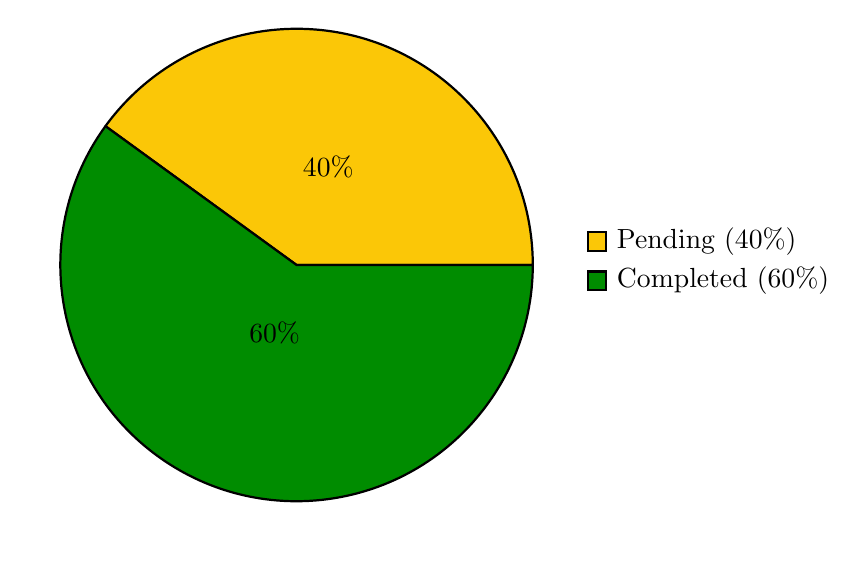
\begin{tikzpicture}
\pie[
    text=legend,
    color={yellow!60!orange, green!55!black},
    radius=3
]{
    40/Pending (40\%),
    60/Completed (60\%)
}
\end{tikzpicture}
\caption{Illustrative Pie Chart -- Task Status Distribution (Pending vs Completed)}
\label{fig:piechart}
\end{figure}

\begin{figure}[h!]
\centering
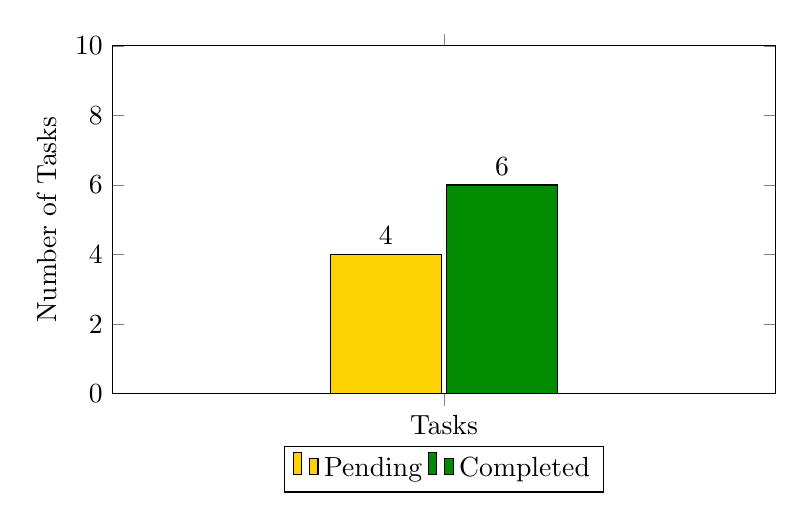
\begin{tikzpicture}
\begin{axis}[
    ybar,
    bar width=40pt,
    width=10cm,
    height=6cm,
    symbolic x coords={Tasks},
    xtick=data,
    ymin=0,
    ymax=10,
    ylabel={Number of Tasks},
    legend style={at={(0.5,-0.15)}, anchor=north, legend columns=-1},
    nodes near coords,
    nodes near coords align={vertical},
    enlarge x limits=0.5
]
\addplot[fill=yellow!70!orange] coordinates {(Tasks,4)};
\addplot[fill=green!55!black]   coordinates {(Tasks,6)};
\legend{Pending, Completed}
\end{axis}
\end{tikzpicture}
\caption{Illustrative Bar Chart -- Pending vs Completed Task Counts}
\label{fig:barchart}
\end{figure}

\section{How the Charts Update}

Because the chart data is rendered server-side via Blade variables, the charts
automatically reflect the current state of the user's tasks every time the page
loads. When the user applies a filter (by status or priority), the filtered
\texttt{\$pending} and \texttt{\$completed} counts passed by the controller update
the chart accordingly, so the visualisation always matches the currently displayed
task list.

% ── Screenshots placeholder ───────────────────────────────

\section{Website Screenshots}

\begin{figure}[h!]
\centering
\includegraphics[width=0.9\textwidth]{login.png}
\caption{Login and Registration}
\label{fig:home}
\end{figure}

\begin{figure}[h!]
\centering
\includegraphics[width=0.9\textwidth]{db.png}
\caption{Main Dashboard -- Task list with statistics, filter controls, and charts}
\label{fig:home}
\end{figure}

\begin{figure}[h!]
\centering
\includegraphics[width=0.9\textwidth]{2.png}
\caption{Add New Task -- Form with title, description, due date, and priority fields}
\label{fig:add}
\end{figure}

\begin{figure}[h!]
\centering
\includegraphics[width=0.9\textwidth]{4.png}
\caption{Edit Task -- Pre-populated form allowing update of all task fields}
\label{fig:edit}
\end{figure}

\begin{figure}[h!]
\centering
\includegraphics[width=0.9\textwidth]{6.png}
\caption{Filter Feature -- Tasks filtered by priority or status using dropdown selectors}
\label{fig:filter}
\end{figure}

\begin{figure}[h!]
\centering
\includegraphics[width=0.9\textwidth]{graph.png}
\caption{Graph Show The complete and pending tasks}
\label{fig:filter}
\end{figure}

\begin{figure}[h!]
\centering
\includegraphics[width=0.9\textwidth]{5.png}
\caption{Task Completed -- Status updated to Completed via toggle button}
\label{fig:completed}
\end{figure}

% ══════════════════════════════════════════════════════════
\chapter*{Conclusion}
\addcontentsline{toc}{chapter}{Conclusion}
% ══════════════════════════════════════════════════════════

This assignment successfully demonstrates the practical implementation of a
web-based To-Do List Management System using the Laravel PHP framework. The
application covers all four CRUD operations in a clean, maintainable codebase
structured according to the MVC design pattern. Additional features -- task
priority levels, due date tracking, status toggling, filter by status and priority,
a real-time statistics dashboard, server-side input validation, and JavaScript
confirmation dialogs -- extend the system beyond a basic data-entry tool into a
usable, real-world task management application.

The integration of \textbf{Laravel Breeze} provides a complete, secure
authentication layer including user registration, login, logout, and password
reset. All task routes are protected by the \texttt{auth} middleware, ensuring that
only authenticated users can access or modify task data. Each user's tasks are
isolated via a \texttt{user\_id} foreign key, giving every registered user a private
and independent task workspace.

The addition of \textbf{Chart.js}-powered pie and bar charts provides users with
an at-a-glance visual summary of their task completion progress. These charts update
dynamically with the server-rendered data on every page load, ensuring the
visualisation always reflects the current state of the user's task list.

Key learning outcomes achieved through this project include:
\begin{itemize}[leftmargin=1.5cm]
    \item Hands-on experience with Laravel routing, controllers, models, and
    Blade views.
    \item Practical understanding of Eloquent ORM for database interactions and
    local query scopes for clean filtering logic.
    \item Implementation of RESTful routing conventions including GET, POST, PUT,
    PATCH, and DELETE HTTP methods.
    \item Integration of \textbf{Laravel Breeze} for full authentication scaffolding
    and understanding of session-based security mechanisms (CSRF protection, password
    hashing, session regeneration, brute-force throttling).
    \item Scoping database queries per authenticated user with foreign key relationships.
    \item Application of server-side validation and flash messaging for user feedback.
    \item Rendering dynamic data charts using \textbf{Chart.js} embedded in Blade views.
    \item Use of Git and GitHub for version control throughout the development cycle.
\end{itemize}

The project can be extended in future work by adding two-factor authentication
(2FA), role-based access control, task categories or tags, pagination for large task
lists, due date reminder notifications, export to CSV/PDF, advanced chart types
(e.g., timeline/Gantt), and deployment to a cloud hosting platform.

% ══════════════════════════════════════════════════════════
% Bibliography
% ══════════════════════════════════════════════════════════
\begin{thebibliography}{9}

\bibitem{laravel}
Laravel LLC. (2024). \textit{Laravel Documentation -- The PHP Framework for Web
Artisans}. Retrieved from \url{https://laravel.com/docs}

\bibitem{breeze}
Laravel LLC. (2024). \textit{Laravel Breeze -- Starter Kit Documentation}.
Retrieved from \url{https://laravel.com/docs/starter-kits#laravel-breeze}

\bibitem{php}
The PHP Group. (2024). \textit{PHP Manual}. Retrieved from
\url{https://www.php.net/manual/en/}

\bibitem{bootstrap}
The Bootstrap Authors. (2024). \textit{Bootstrap 5 Documentation}. Retrieved from
\url{https://getbootstrap.com/docs/5.0/}

\bibitem{chartjs}
Chart.js Contributors. (2024). \textit{Chart.js Documentation}. Retrieved from
\url{https://www.chartjs.org/docs/latest/}

\bibitem{mysql}
Oracle Corporation. (2024). \textit{MySQL 8.0 Reference Manual}. Retrieved from
\url{https://dev.mysql.com/doc/refman/8.0/en/}

\bibitem{mvc}
Gamma, E., Helm, R., Johnson, R., \& Vlissides, J. (1994). \textit{Design Patterns:
Elements of Reusable Object-Oriented Software}. Addison-Wesley.

\end{thebibliography}

\end{document}